\documentclass[12pt,a4paper]{article}
\usepackage[UTF8]{ctex}
\usepackage{amsmath,amssymb}
\usepackage{xcolor}
\usepackage{hyperref}
\usepackage{geometry}
\usepackage{graphicx}
\geometry{margin=2.5cm}

\title{Syndrome Decoding / 伴随子解码}
\author{QuoNic}
\date{}

\begin{document}
\maketitle

\begin{center}
\textbf{Error Correction / 纠错} | 难度：中级 | 预计时间：15 分钟
\end{center}

\tableofcontents
\newpage

\section{为什么需要？}

伴随子解码是量子纠错中的核心步骤，用于检测和纠正错误。

\subsection{经典局限}
\begin{itemize}
  \item 经典纠错码不能直接用于量子系统
  \item 量子纠错需要特殊的解码方式
\end{itemize}

\subsection{量子优势}
\begin{itemize}
  \item 伴随子解码可以高效检测量子错误
  \item 不会破坏量子态
  \item 是量子纠错的核心步骤
\end{itemize}

\subsection{实际应用}
\begin{itemize}
  \item 量子纠错
  \item 量子密钥分发
  \item 量子计算
\end{itemize}

\section{快速上手}

\begin{verbatim}
from quonic.qec import syndrome

# 伴随子解码
result = syndrome(code='bit_flip', error='X', position=1)
print(f'Syndrome: {result.syndrome}')
print(f'Correction: {result.correction}')
\end{verbatim}

\textbf{预期输出}：
\begin{verbatim}
Syndrome: [1, 0]
Correction: X on qubit 1
\end{verbatim}

\section{原理详解}

\subsection{电路图}

\begin{center}
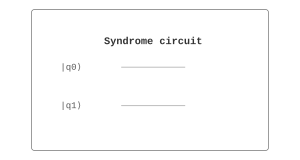
\includegraphics[width=0.6\textwidth]{../../images/syndrome_circuit.svg}
\end{center}

\subsection{数学推导}

伴随子测量：
\begin{equation}
s_i = \langle\psi|g_i|\psi\rangle
\end{equation}

其中 $g_i$ 是稳定子生成元。

\textbf{解码}：
\begin{equation}
s = (s_1, s_2, \ldots, s_{n-k})
\end{equation}

\textbf{纠正}：
\begin{equation}
E \to E \cdot C_s
\end{equation}

其中 $C_s$ 是对应伴随子 $s$ 的纠正算子。

\subsection{几何解释}

伴随子解码在群空间中检测错误。伴随子是错误的"指纹"，不同的错误有不同的伴随子。

\section{代码详解}

\begin{verbatim}
from quonic.qec import syndrome

# syndrome(code, error, position)
# code: 纠错码类型
# error: 错误类型
# position: 错误位置

result = syndrome(
    code='bit_flip',
    error='X',
    position=1
)

# result.syndrome: 伴随子
# result.correction: 纠正操作
# result.circuit: 解码电路
print(f'Syndrome: {result.syndrome}')
print(f'Correction: {result.correction}')
\end{verbatim}

\section{进阶用法}

\subsection{场景 1：不同错误类型}

\begin{verbatim}
from quonic.qec import syndrome

# 不同错误类型
for error in ['X', 'Z', 'Y']:
    result = syndrome(code='bit_flip', error=error, position=0)
    print(f'{error} error: Syndrome={result.syndrome}')
\end{verbatim}

\subsection{场景 2：不同纠错码}

\begin{verbatim}
from quonic.qec import syndrome

# 不同纠错码
for code in ['bit_flip', 'phase_flip', 'steane']:
    result = syndrome(code=code, error='X', position=0)
    print(f'{code}: Syndrome={result.syndrome}')
\end{verbatim}

\subsection{场景 3：多比特错误}

\begin{verbatim}
from quonic.qec import syndrome

# 多比特错误
result = syndrome(code='bit_flip', error='X', position=[0, 2])
print(f'Syndrome: {result.syndrome}')
print(f'Correction: {result.correction}')
\end{verbatim}

\section{适用场景}

\subsection{量子纠错}

伴随子解码是量子纠错的核心步骤。通过测量伴随子，可以检测和纠正量子错误。

\subsection{量子密钥分发}

伴随子解码可以用于量子密钥分发中的错误检测。伴随子测量可以检测窃听行为。

\subsection{量子计算}

伴随子解码可以用于容错量子计算。伴随子测量可以保护量子信息免受噪声影响。

\section{常见问题}

\subsection{伴随子解码和经典解码有什么区别？}

伴随子解码不会破坏量子态，经典解码会破坏信息。

\subsection{伴随子解码的精度如何？}

伴随子解码的精度取决于纠错码的码距。码距越大，纠错能力越强。

\section{学习路径}

\subsection{前置知识}
\begin{itemize}
  \item 量子纠错码
  \item 稳定子形式
  \item 量子测量
\end{itemize}

\subsection{继续学习}
\begin{itemize}
  \item 容错量子计算
  \item 量子纠错码设计
  \item 量子硬件
\end{itemize}

\section{完整示例代码}

\subsection{示例 1：基本伴随子解码}

\begin{verbatim}
from quonic.qec import syndrome

result = syndrome(code='bit_flip', error='X', position=1)
print(f'Syndrome: {result.syndrome}')
\end{verbatim}

\section{下载}

\begin{itemize}
  \item [syndrome.py](https://github.com/ChrisLee0721/QuoNic/blob/main/examples/syndrome/syndrome.py)
\end{itemize}

\end{document}
